% !TEX root = robobrain.tex
\section{Discussion and Conclusion}
The \robobrain{} graph currently has 44347 nodes (concepts) and 98465 edges (relations). The knowledge in the graph is obtained from the Internet sources and through the \robobrain{} project partners. For the success of many robotics application it is important to relate and connect the concepts from these different knowledge sources. In order to empirically evaluate the connectivity of  concepts in \robobrain{}, we plot the degree distribution of the \robobrain{} graph and compare it with the degree distribution of independent knowledge sources (Figure~\ref{degDis}).
The graph of independent knowledge sources is the union of each knowledge source, which have nodes from all the projects and the edges only between the nodes from the same project.
As shown in the Figure~\ref{degDis}, \robobrain{} successfully connects projects and increases the average degree per-node by $0.8$.
\begin{figure}[h!]
 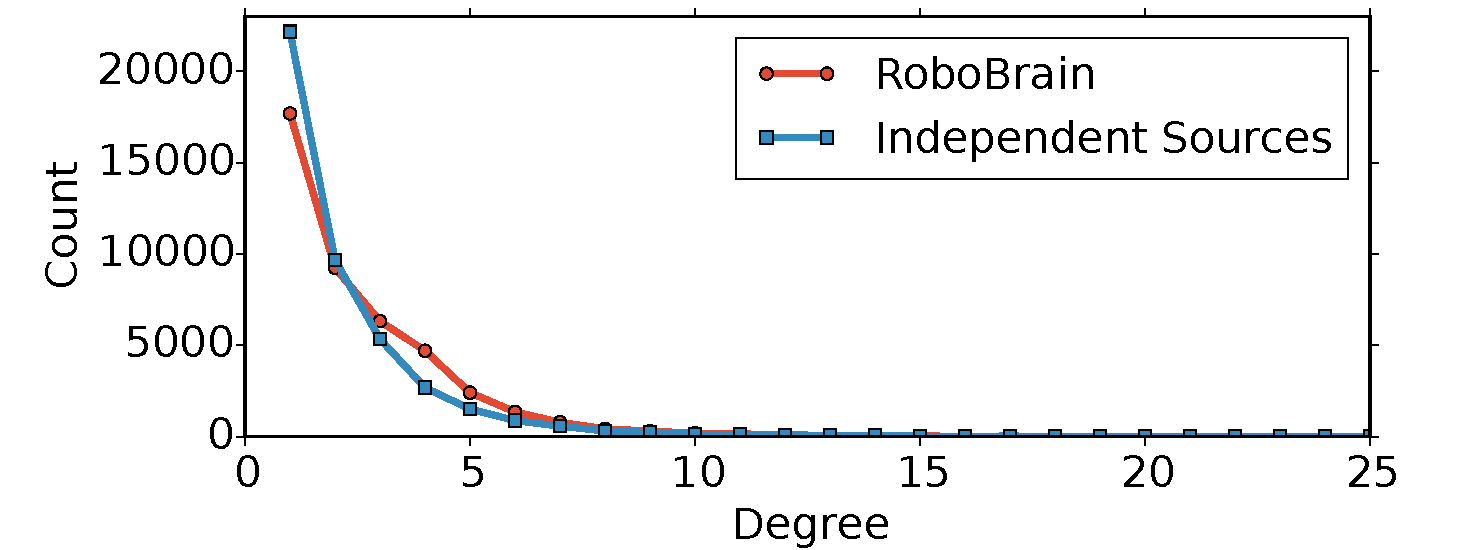
\includegraphics[width=\linewidth, height=1.5in]{Image/deg}
 \caption{Degree distribution of \robobrain{} and the union of independent knowledge sources.
 For the case of independent sources, we only consider the edges between nodes from the same
 source. \robobrain{} connects different projects successfully: number of nodes with degree 1 and 2 decrease and  nodes with degree 3 and more increase.}
% \vspace*{\captionReduceTop}
\label{degDis}
\vskip -.1in
\end{figure}
The \robobrain{} graph has fifteen thousand nodes with degree one. Most of the nodes with a single degree come from the Internet sources such as Wikipedia  and WordNet. These nodes are not directly related to the physical world and represent abstract concepts like political ideas, categories of art, etc.

In this paper we described different aspects and technical challenges in building \robobrain{} knowledge engine. \robobrain{} represents multiple data modalities from various sources, and connects them to get an overall rich graph representation.  We presented an overview of the \robobrain{} large-scale system architecture and developed the Robot Query Library (RQL) for robots to use \robobrain{}. We illustrated robotics applications of anticipation, natural language grounding, and path planning as simple RQL queries to \robobrain{}. We also showed in experiments that sharing knowledge through \robobrain{} improves existing path planning and natural language grounding algorithms.
 \robobrain{} is an ongoing effort where we are collaborating with different research groups. We are working on improving different aspects such as learning from crowd-sourcing feedback, inference methods over the graph for discovering new relations between concepts, and expanding \robobrain{} to new robotics applications.

\iffalse
\robobrain{} is an ongoing effort, where we are constantly improving different aspects of the work.
% We are improving the system architecture and expanding RQL to support scaling to even larger
% knowledge sources (e.g., millions of videos).
% Furthermore,  w
We have several ongoing research efforts that include achieving
better disambiguation and improving never-ending learning abilities.
More importantly, we are constantly expanding the set of our \robobrain{} research partners.
This will not only improve the abilities of their robots, but also their contribution of knowledge
to \robobrain{} will help other researchers in the robotics community at large.
\fi
